\documentclass[twoside]{book}

% Packages required by doxygen
\usepackage{calc}
\usepackage{doxygen}
\usepackage{graphicx}
\usepackage[utf8]{inputenc}
\usepackage{makeidx}
\usepackage{multicol}
\usepackage{multirow}
\usepackage{textcomp}
\usepackage[table]{xcolor}

% Font selection
\usepackage[T1]{fontenc}
\usepackage{mathptmx}
\usepackage[scaled=.90]{helvet}
\usepackage{courier}
\usepackage{amssymb}
\usepackage{sectsty}
\renewcommand{\familydefault}{\sfdefault}
\allsectionsfont{%
  \fontseries{bc}\selectfont%
  \color{darkgray}%
}
\renewcommand{\DoxyLabelFont}{%
  \fontseries{bc}\selectfont%
  \color{darkgray}%
}

% Page & text layout
\usepackage{geometry}
\geometry{%
  a4paper,%
  top=2.5cm,%
  bottom=2.5cm,%
  left=2.5cm,%
  right=2.5cm%
}
\tolerance=750
\hfuzz=15pt
\hbadness=750
\setlength{\emergencystretch}{15pt}
\setlength{\parindent}{0cm}
\setlength{\parskip}{0.2cm}
\makeatletter
\renewcommand{\paragraph}{%
  \@startsection{paragraph}{4}{0ex}{-1.0ex}{1.0ex}{%
    \normalfont\normalsize\bfseries\SS@parafont%
  }%
}
\renewcommand{\subparagraph}{%
  \@startsection{subparagraph}{5}{0ex}{-1.0ex}{1.0ex}{%
    \normalfont\normalsize\bfseries\SS@subparafont%
  }%
}
\makeatother

% Headers & footers
\usepackage{fancyhdr}
\pagestyle{fancyplain}
\fancyhead[LE]{\fancyplain{}{\bfseries\thepage}}
\fancyhead[CE]{\fancyplain{}{}}
\fancyhead[RE]{\fancyplain{}{\bfseries\leftmark}}
\fancyhead[LO]{\fancyplain{}{\bfseries\rightmark}}
\fancyhead[CO]{\fancyplain{}{}}
\fancyhead[RO]{\fancyplain{}{\bfseries\thepage}}
\fancyfoot[LE]{\fancyplain{}{}}
\fancyfoot[CE]{\fancyplain{}{}}
\fancyfoot[RE]{\fancyplain{}{\bfseries\scriptsize Generated on Sun Dec 21 2014 14\-:50\-:37 for Relax\-Auto by Doxygen }}
\fancyfoot[LO]{\fancyplain{}{\bfseries\scriptsize Generated on Sun Dec 21 2014 14\-:50\-:37 for Relax\-Auto by Doxygen }}
\fancyfoot[CO]{\fancyplain{}{}}
\fancyfoot[RO]{\fancyplain{}{}}
\renewcommand{\footrulewidth}{0.4pt}
\renewcommand{\chaptermark}[1]{%
  \markboth{#1}{}%
}
\renewcommand{\sectionmark}[1]{%
  \markright{\thesection\ #1}%
}

% Indices & bibliography
\usepackage{natbib}
\usepackage[titles]{tocloft}
\setcounter{tocdepth}{3}
\setcounter{secnumdepth}{5}
\makeindex

% Hyperlinks (required, but should be loaded last)
\usepackage{ifpdf}
\ifpdf
  \usepackage[pdftex,pagebackref=true]{hyperref}
\else
  \usepackage[ps2pdf,pagebackref=true]{hyperref}
\fi
\hypersetup{%
  colorlinks=true,%
  linkcolor=blue,%
  citecolor=blue,%
  unicode%
}

% Custom commands
\newcommand{\clearemptydoublepage}{%
  \newpage{\pagestyle{empty}\cleardoublepage}%
}


%===== C O N T E N T S =====

\begin{document}

% Titlepage & ToC
\hypersetup{pageanchor=false}
\pagenumbering{roman}
\begin{titlepage}
\vspace*{7cm}
\begin{center}%
{\Large Relax\-Auto }\\
\vspace*{1cm}
{\large Generated by Doxygen 1.8.6}\\
\vspace*{0.5cm}
{\small Sun Dec 21 2014 14:50:37}\\
\end{center}
\end{titlepage}
\clearemptydoublepage
\tableofcontents
\clearemptydoublepage
\pagenumbering{arabic}
\hypersetup{pageanchor=true}

%--- Begin generated contents ---
\chapter{Namespace Index}
\section{Namespace List}
Here is a list of all documented namespaces with brief descriptions\-:\begin{DoxyCompactList}
\item\contentsline{section}{\hyperlink{namespaceattributes}{attributes} \\*\hyperlink{classattributes_1_1_attribute}{Attribute} classes }{\pageref{namespaceattributes}}{}
\item\contentsline{section}{\hyperlink{namespaceauto}{auto} \\*Mostly an initialization file }{\pageref{namespaceauto}}{}
\item\contentsline{section}{\hyperlink{namespacemain}{main} \\*Main file where the automation takes place }{\pageref{namespacemain}}{}
\end{DoxyCompactList}

\chapter{Hierarchical Index}
\section{Class Hierarchy}
This inheritance list is sorted roughly, but not completely, alphabetically\-:\begin{DoxyCompactList}
\item \contentsline{section}{attributes.\-Attribute}{\pageref{classattributes_1_1_attribute}}{}
\begin{DoxyCompactList}
\item \contentsline{section}{attributes.\-Boolean\-Attribute}{\pageref{classattributes_1_1_boolean_attribute}}{}
\item \contentsline{section}{attributes.\-Float\-Attribute}{\pageref{classattributes_1_1_float_attribute}}{}
\item \contentsline{section}{attributes.\-Int\-Attribute}{\pageref{classattributes_1_1_int_attribute}}{}
\end{DoxyCompactList}
\item \contentsline{section}{auto.\-Auto}{\pageref{classauto_1_1_auto}}{}
\end{DoxyCompactList}

\chapter{Class Index}
\section{Class List}
Here are the classes, structs, unions and interfaces with brief descriptions\-:\begin{DoxyCompactList}
\item\contentsline{section}{\hyperlink{classattributes_1_1_attribute}{attributes.\-Attribute} \\*Allows the inclusion of new attributes with a fairly standard way of initialization }{\pageref{classattributes_1_1_attribute}}{}
\item\contentsline{section}{\hyperlink{classauto_1_1_auto}{auto.\-Auto} \\*Initializes Attribute objects and provides several methods that make automation easier }{\pageref{classauto_1_1_auto}}{}
\item\contentsline{section}{\hyperlink{classattributes_1_1_boolean_attribute}{attributes.\-Boolean\-Attribute} \\*Subclass of the \hyperlink{classattributes_1_1_attribute}{Attribute} Class }{\pageref{classattributes_1_1_boolean_attribute}}{}
\item\contentsline{section}{\hyperlink{classattributes_1_1_float_attribute}{attributes.\-Float\-Attribute} \\*Subclass of the \hyperlink{classattributes_1_1_attribute}{Attribute} Class }{\pageref{classattributes_1_1_float_attribute}}{}
\item\contentsline{section}{\hyperlink{classattributes_1_1_int_attribute}{attributes.\-Int\-Attribute} \\*Subclass of the \hyperlink{classattributes_1_1_attribute}{Attribute} Class }{\pageref{classattributes_1_1_int_attribute}}{}
\end{DoxyCompactList}

\chapter{Namespace Documentation}
\hypertarget{namespaceattributes}{\section{attributes Namespace Reference}
\label{namespaceattributes}\index{attributes@{attributes}}
}


\hyperlink{classattributes_1_1_attribute}{Attribute} classes.  


\subsection*{Classes}
\begin{DoxyCompactItemize}
\item 
class \hyperlink{classattributes_1_1_attribute}{Attribute}
\begin{DoxyCompactList}\small\item\em Allows the inclusion of new attributes with a fairly standard way of initialization. \end{DoxyCompactList}\item 
class \hyperlink{classattributes_1_1_int_attribute}{Int\-Attribute}
\begin{DoxyCompactList}\small\item\em Subclass of the \hyperlink{classattributes_1_1_attribute}{Attribute} Class. \end{DoxyCompactList}\item 
class \hyperlink{classattributes_1_1_float_attribute}{Float\-Attribute}
\begin{DoxyCompactList}\small\item\em Subclass of the \hyperlink{classattributes_1_1_attribute}{Attribute} Class. \end{DoxyCompactList}\item 
class \hyperlink{classattributes_1_1_boolean_attribute}{Boolean\-Attribute}
\begin{DoxyCompactList}\small\item\em Subclass of the \hyperlink{classattributes_1_1_attribute}{Attribute} Class. \end{DoxyCompactList}\end{DoxyCompactItemize}


\subsection{Detailed Description}
\hyperlink{classattributes_1_1_attribute}{Attribute} classes. 
\hypertarget{namespaceauto}{\section{auto Namespace Reference}
\label{namespaceauto}\index{auto@{auto}}
}


Mostly an initialization file.  


\subsection*{Classes}
\begin{DoxyCompactItemize}
\item 
class \hyperlink{classauto_1_1_auto}{Auto}
\begin{DoxyCompactList}\small\item\em Initializes Attribute objects and provides several methods that make automation easier. \end{DoxyCompactList}\end{DoxyCompactItemize}
\subsection*{Functions}
\begin{DoxyCompactItemize}
\item 
def \hyperlink{namespaceauto_a53915090ec037344b60988bfa6fbe36b}{check\-\_\-volume\-\_\-difference}
\begin{DoxyCompactList}\small\item\em Checks the current volume difference. \end{DoxyCompactList}\item 
def \hyperlink{namespaceauto_a2bd6aa728264fc3b4ce4599bd4c0dd99}{get\-\_\-volumes}
\begin{DoxyCompactList}\small\item\em Gets two volumes. \end{DoxyCompactList}\item 
def \hyperlink{namespaceauto_a22c2b861da246cc96b2092c5ddb2a267}{get\-\_\-volume\-\_\-difference}
\begin{DoxyCompactList}\small\item\em Determines the absolute volume of a volume list. \end{DoxyCompactList}\item 
def \hyperlink{namespaceauto_a54eadb35ea17c33902b8ccce7fcfb203}{find\-\_\-first\-\_\-last\-\_\-volume}
\begin{DoxyCompactList}\small\item\em Finds the first and last volume in a list of strings. \end{DoxyCompactList}\item 
def \hyperlink{namespaceauto_a27348316feee628368d1407f6f54a94d}{find\-\_\-min\-\_\-max\-\_\-volume}
\begin{DoxyCompactList}\small\item\em Finds the maximum and minimum volume in a list of strings. \end{DoxyCompactList}\end{DoxyCompactItemize}


\subsection{Detailed Description}
Mostly an initialization file. 

\subsection{Function Documentation}
\hypertarget{namespaceauto_a53915090ec037344b60988bfa6fbe36b}{\index{auto@{auto}!check\-\_\-volume\-\_\-difference@{check\-\_\-volume\-\_\-difference}}
\index{check\-\_\-volume\-\_\-difference@{check\-\_\-volume\-\_\-difference}!auto@{auto}}
\subsubsection[{check\-\_\-volume\-\_\-difference}]{\setlength{\rightskip}{0pt plus 5cm}def auto.\-check\-\_\-volume\-\_\-difference (
\begin{DoxyParamCaption}
\item[{}]{obj}
\end{DoxyParamCaption}
)}}\label{namespaceauto_a53915090ec037344b60988bfa6fbe36b}


Checks the current volume difference. 


\begin{DoxyParams}{Parameters}
{\em \hyperlink{classauto_1_1_auto}{Auto}} & Object\\
\hline
\end{DoxyParams}
\begin{DoxyReturn}{Returns}
Returns a boolean
\end{DoxyReturn}

\begin{DoxyRetVals}{Return values}
{\em False} & if the volume difference is greater than the requirements. \\
\hline
{\em True} & if the volume difference meets requirements \\
\hline
\end{DoxyRetVals}
\hypertarget{namespaceauto_a54eadb35ea17c33902b8ccce7fcfb203}{\index{auto@{auto}!find\-\_\-first\-\_\-last\-\_\-volume@{find\-\_\-first\-\_\-last\-\_\-volume}}
\index{find\-\_\-first\-\_\-last\-\_\-volume@{find\-\_\-first\-\_\-last\-\_\-volume}!auto@{auto}}
\subsubsection[{find\-\_\-first\-\_\-last\-\_\-volume}]{\setlength{\rightskip}{0pt plus 5cm}def auto.\-find\-\_\-first\-\_\-last\-\_\-volume (
\begin{DoxyParamCaption}
\item[{}]{lines, }
\item[{}]{Verbose}
\end{DoxyParamCaption}
)}}\label{namespaceauto_a54eadb35ea17c33902b8ccce7fcfb203}


Finds the first and last volume in a list of strings. 


\begin{DoxyParams}{Parameters}
{\em lines} & is a list of strings \\
\hline
{\em Verbose} & is boolean variable\\
\hline
\end{DoxyParams}
\begin{DoxyReturn}{Returns}
returns a list of floats 
\end{DoxyReturn}
\hypertarget{namespaceauto_a27348316feee628368d1407f6f54a94d}{\index{auto@{auto}!find\-\_\-min\-\_\-max\-\_\-volume@{find\-\_\-min\-\_\-max\-\_\-volume}}
\index{find\-\_\-min\-\_\-max\-\_\-volume@{find\-\_\-min\-\_\-max\-\_\-volume}!auto@{auto}}
\subsubsection[{find\-\_\-min\-\_\-max\-\_\-volume}]{\setlength{\rightskip}{0pt plus 5cm}def auto.\-find\-\_\-min\-\_\-max\-\_\-volume (
\begin{DoxyParamCaption}
\item[{}]{lines, }
\item[{}]{Verbose}
\end{DoxyParamCaption}
)}}\label{namespaceauto_a27348316feee628368d1407f6f54a94d}


Finds the maximum and minimum volume in a list of strings. 


\begin{DoxyParams}{Parameters}
{\em lines} & is a list of strings \\
\hline
{\em Verbose} & is a boolean variable that determines whether the function should be verbose\\
\hline
\end{DoxyParams}
\begin{DoxyReturn}{Returns}
returns a list, with the max volume being the first index. 
\end{DoxyReturn}
\hypertarget{namespaceauto_a22c2b861da246cc96b2092c5ddb2a267}{\index{auto@{auto}!get\-\_\-volume\-\_\-difference@{get\-\_\-volume\-\_\-difference}}
\index{get\-\_\-volume\-\_\-difference@{get\-\_\-volume\-\_\-difference}!auto@{auto}}
\subsubsection[{get\-\_\-volume\-\_\-difference}]{\setlength{\rightskip}{0pt plus 5cm}def auto.\-get\-\_\-volume\-\_\-difference (
\begin{DoxyParamCaption}
\item[{}]{volume}
\end{DoxyParamCaption}
)}}\label{namespaceauto_a22c2b861da246cc96b2092c5ddb2a267}


Determines the absolute volume of a volume list. 


\begin{DoxyParams}{Parameters}
{\em float} & list with two members\\
\hline
\end{DoxyParams}
\begin{DoxyReturn}{Returns}
Absolute value of the difference between the two floats in the list 
\end{DoxyReturn}
\hypertarget{namespaceauto_a2bd6aa728264fc3b4ce4599bd4c0dd99}{\index{auto@{auto}!get\-\_\-volumes@{get\-\_\-volumes}}
\index{get\-\_\-volumes@{get\-\_\-volumes}!auto@{auto}}
\subsubsection[{get\-\_\-volumes}]{\setlength{\rightskip}{0pt plus 5cm}def auto.\-get\-\_\-volumes (
\begin{DoxyParamCaption}
\item[{}]{obj}
\end{DoxyParamCaption}
)}}\label{namespaceauto_a2bd6aa728264fc3b4ce4599bd4c0dd99}


Gets two volumes. 


\begin{DoxyParams}{Parameters}
{\em \hyperlink{classauto_1_1_auto}{Auto}} & Object\\
\hline
\end{DoxyParams}
\begin{DoxyReturn}{Returns}
returns a list of floats. 
\end{DoxyReturn}

\hypertarget{namespacemain}{\section{main Namespace Reference}
\label{namespacemain}\index{main@{main}}
}


main file where the automation takes place.  


\subsection*{Functions}
\begin{DoxyCompactItemize}
\item 
\hypertarget{namespacemain_a021bfca46dd0435fb213d09cf10db27e}{def {\bfseries main}}\label{namespacemain_a021bfca46dd0435fb213d09cf10db27e}

\item 
def \hyperlink{namespacemain_a28b1b2d246ad4083aadee297737987df}{run\-\_\-automation}
\begin{DoxyCompactList}\small\item\em The primary function for running the volume automation logic. \end{DoxyCompactList}\item 
def \hyperlink{namespacemain_aee361eab1cf2faee05ed088fecf8e20c}{check\-\_\-for\-\_\-errors}
\begin{DoxyCompactList}\small\item\em Checks for errors within the volume relaxation automation. \end{DoxyCompactList}\item 
\hypertarget{namespacemain_adde7593aad11ae1c86dce6604692aa30}{def {\bfseries print\-\_\-lines}}\label{namespacemain_adde7593aad11ae1c86dce6604692aa30}

\end{DoxyCompactItemize}


\subsection{Detailed Description}
main file where the automation takes place. Usually this code will not be modified, and should not be modified unless you plan on editing the automation of the program itself. 

\subsection{Function Documentation}
\hypertarget{namespacemain_aee361eab1cf2faee05ed088fecf8e20c}{\index{main@{main}!check\-\_\-for\-\_\-errors@{check\-\_\-for\-\_\-errors}}
\index{check\-\_\-for\-\_\-errors@{check\-\_\-for\-\_\-errors}!main@{main}}
\subsubsection[{check\-\_\-for\-\_\-errors}]{\setlength{\rightskip}{0pt plus 5cm}def main.\-check\-\_\-for\-\_\-errors (
\begin{DoxyParamCaption}
\item[{}]{obj}
\end{DoxyParamCaption}
)}}\label{namespacemain_aee361eab1cf2faee05ed088fecf8e20c}


Checks for errors within the volume relaxation automation. 


\begin{DoxyParams}{Parameters}
{\em Auto} & object variable \\
\hline
\end{DoxyParams}
\hypertarget{namespacemain_a28b1b2d246ad4083aadee297737987df}{\index{main@{main}!run\-\_\-automation@{run\-\_\-automation}}
\index{run\-\_\-automation@{run\-\_\-automation}!main@{main}}
\subsubsection[{run\-\_\-automation}]{\setlength{\rightskip}{0pt plus 5cm}def main.\-run\-\_\-automation (
\begin{DoxyParamCaption}
\item[{}]{obj}
\end{DoxyParamCaption}
)}}\label{namespacemain_a28b1b2d246ad4083aadee297737987df}


The primary function for running the volume automation logic. 


\begin{DoxyParams}{Parameters}
{\em Auto} & Object variable\\
\hline
\end{DoxyParams}
This function should only ever be called once during the entire execution of the program. 
\chapter{Class Documentation}
\hypertarget{classattributes_1_1_attribute}{\section{attributes.\-Attribute Class Reference}
\label{classattributes_1_1_attribute}\index{attributes.\-Attribute@{attributes.\-Attribute}}
}


Allows the inclusion of new attributes with a fairly standard way of initialization.  


Inheritance diagram for attributes.\-Attribute\-:\begin{figure}[H]
\begin{center}
\leavevmode
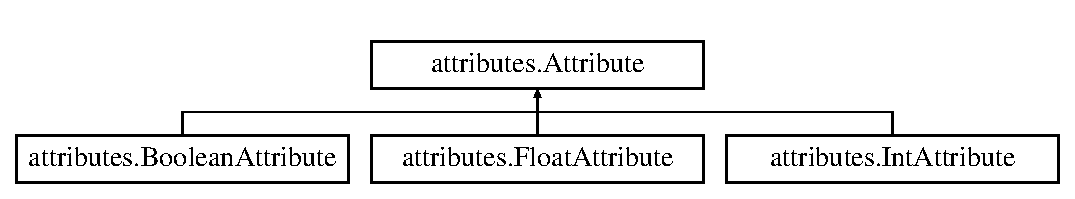
\includegraphics[height=2.000000cm]{classattributes_1_1_attribute}
\end{center}
\end{figure}
\subsection*{Public Member Functions}
\begin{DoxyCompactItemize}
\item 
def \hyperlink{classattributes_1_1_attribute_afe761453b838f336a71de981967a1196}{\-\_\-\-\_\-init\-\_\-\-\_\-}
\begin{DoxyCompactList}\small\item\em Class constructor. \end{DoxyCompactList}\item 
def \hyperlink{classattributes_1_1_attribute_a78546761ea790b58b9bf3746e38a59ae}{initialize\-\_\-attribute}
\begin{DoxyCompactList}\small\item\em Initializes the variable Attribute\-String. \end{DoxyCompactList}\item 
def \hyperlink{classattributes_1_1_attribute_aad32ba32a123223d68222083443df8ff}{set\-\_\-to\-\_\-default\-\_\-attribute}
\begin{DoxyCompactList}\small\item\em sets the variable Attribute\-String to the variable Default\-Attribute \end{DoxyCompactList}\item 
def \hyperlink{classattributes_1_1_attribute_a49ed6d4ece850ee63616ecddb95f7e34}{set\-\_\-attribute}
\begin{DoxyCompactList}\small\item\em sets the variable Attribute\-String to the passed variable attribute \end{DoxyCompactList}\item 
def \hyperlink{classattributes_1_1_attribute_a0ec4eaea8ac789e42e83a65a24d82752}{set\-\_\-boolean}
\begin{DoxyCompactList}\small\item\em sets the object variable boolean to the passed boolean variable \end{DoxyCompactList}\item 
def \hyperlink{classattributes_1_1_attribute_a5897c5790735326e884f656152b598d9}{get\-\_\-name}
\item 
def \hyperlink{classattributes_1_1_attribute_a1ce4013ad2db9bde281140d35306b656}{get\-\_\-attribute}
\item 
def \hyperlink{classattributes_1_1_attribute_a3ff8dacaff71408ae6991458b38255c8}{get\-\_\-boolean}
\end{DoxyCompactItemize}
\subsection*{Public Attributes}
\begin{DoxyCompactItemize}
\item 
\hypertarget{classattributes_1_1_attribute_abd2b00a6f6fd6b42c304f3f625786da3}{{\bfseries name}}\label{classattributes_1_1_attribute_abd2b00a6f6fd6b42c304f3f625786da3}

\item 
\hypertarget{classattributes_1_1_attribute_ad4773ea8c8db55052869218876d48f5e}{{\bfseries Attribute\-String}}\label{classattributes_1_1_attribute_ad4773ea8c8db55052869218876d48f5e}

\item 
\hypertarget{classattributes_1_1_attribute_ae123bfe48f8ae7a0a8532d02c5bc4432}{{\bfseries boolean}}\label{classattributes_1_1_attribute_ae123bfe48f8ae7a0a8532d02c5bc4432}

\item 
\hypertarget{classattributes_1_1_attribute_ac547a8f17642b92159277f3d0e88053f}{{\bfseries Default\-Attribute}}\label{classattributes_1_1_attribute_ac547a8f17642b92159277f3d0e88053f}

\end{DoxyCompactItemize}


\subsection{Detailed Description}
Allows the inclusion of new attributes with a fairly standard way of initialization. 



\subsection{Constructor \& Destructor Documentation}
\hypertarget{classattributes_1_1_attribute_afe761453b838f336a71de981967a1196}{\index{attributes\-::\-Attribute@{attributes\-::\-Attribute}!\-\_\-\-\_\-init\-\_\-\-\_\-@{\-\_\-\-\_\-init\-\_\-\-\_\-}}
\index{\-\_\-\-\_\-init\-\_\-\-\_\-@{\-\_\-\-\_\-init\-\_\-\-\_\-}!attributes::Attribute@{attributes\-::\-Attribute}}
\subsubsection[{\-\_\-\-\_\-init\-\_\-\-\_\-}]{\setlength{\rightskip}{0pt plus 5cm}def attributes.\-Attribute.\-\_\-\-\_\-init\-\_\-\-\_\- (
\begin{DoxyParamCaption}
\item[{}]{self, }
\item[{}]{name, }
\item[{}]{Default\-Attribute = {\ttfamily False}}
\end{DoxyParamCaption}
)}}\label{classattributes_1_1_attribute_afe761453b838f336a71de981967a1196}


Class constructor. 

You can pass a default attribute to your object in the event that there is a syntax error within the autoinit config file. This allows for continued execution, where there could have been potentially runtime errors. 

\subsection{Member Function Documentation}
\hypertarget{classattributes_1_1_attribute_a1ce4013ad2db9bde281140d35306b656}{\index{attributes\-::\-Attribute@{attributes\-::\-Attribute}!get\-\_\-attribute@{get\-\_\-attribute}}
\index{get\-\_\-attribute@{get\-\_\-attribute}!attributes::Attribute@{attributes\-::\-Attribute}}
\subsubsection[{get\-\_\-attribute}]{\setlength{\rightskip}{0pt plus 5cm}def attributes.\-Attribute.\-get\-\_\-attribute (
\begin{DoxyParamCaption}
\item[{}]{self}
\end{DoxyParamCaption}
)}}\label{classattributes_1_1_attribute_a1ce4013ad2db9bde281140d35306b656}
\begin{DoxyReturn}{Returns}
returns the variable Attribute\-String 
\end{DoxyReturn}
\hypertarget{classattributes_1_1_attribute_a3ff8dacaff71408ae6991458b38255c8}{\index{attributes\-::\-Attribute@{attributes\-::\-Attribute}!get\-\_\-boolean@{get\-\_\-boolean}}
\index{get\-\_\-boolean@{get\-\_\-boolean}!attributes::Attribute@{attributes\-::\-Attribute}}
\subsubsection[{get\-\_\-boolean}]{\setlength{\rightskip}{0pt plus 5cm}def attributes.\-Attribute.\-get\-\_\-boolean (
\begin{DoxyParamCaption}
\item[{}]{self}
\end{DoxyParamCaption}
)}}\label{classattributes_1_1_attribute_a3ff8dacaff71408ae6991458b38255c8}
\begin{DoxyReturn}{Returns}
returns the variable boolean 
\end{DoxyReturn}
\hypertarget{classattributes_1_1_attribute_a5897c5790735326e884f656152b598d9}{\index{attributes\-::\-Attribute@{attributes\-::\-Attribute}!get\-\_\-name@{get\-\_\-name}}
\index{get\-\_\-name@{get\-\_\-name}!attributes::Attribute@{attributes\-::\-Attribute}}
\subsubsection[{get\-\_\-name}]{\setlength{\rightskip}{0pt plus 5cm}def attributes.\-Attribute.\-get\-\_\-name (
\begin{DoxyParamCaption}
\item[{}]{self}
\end{DoxyParamCaption}
)}}\label{classattributes_1_1_attribute_a5897c5790735326e884f656152b598d9}
\begin{DoxyReturn}{Returns}
returns the name of the \hyperlink{classattributes_1_1_attribute}{Attribute} object 
\end{DoxyReturn}
\hypertarget{classattributes_1_1_attribute_a78546761ea790b58b9bf3746e38a59ae}{\index{attributes\-::\-Attribute@{attributes\-::\-Attribute}!initialize\-\_\-attribute@{initialize\-\_\-attribute}}
\index{initialize\-\_\-attribute@{initialize\-\_\-attribute}!attributes::Attribute@{attributes\-::\-Attribute}}
\subsubsection[{initialize\-\_\-attribute}]{\setlength{\rightskip}{0pt plus 5cm}def attributes.\-Attribute.\-initialize\-\_\-attribute (
\begin{DoxyParamCaption}
\item[{}]{self, }
\item[{}]{string}
\end{DoxyParamCaption}
)}}\label{classattributes_1_1_attribute_a78546761ea790b58b9bf3746e38a59ae}


Initializes the variable Attribute\-String. 

This is the method that shouldd be called, instead of set\-\_\-attribute \hypertarget{classattributes_1_1_attribute_a49ed6d4ece850ee63616ecddb95f7e34}{\index{attributes\-::\-Attribute@{attributes\-::\-Attribute}!set\-\_\-attribute@{set\-\_\-attribute}}
\index{set\-\_\-attribute@{set\-\_\-attribute}!attributes::Attribute@{attributes\-::\-Attribute}}
\subsubsection[{set\-\_\-attribute}]{\setlength{\rightskip}{0pt plus 5cm}def attributes.\-Attribute.\-set\-\_\-attribute (
\begin{DoxyParamCaption}
\item[{}]{self, }
\item[{}]{attribute}
\end{DoxyParamCaption}
)}}\label{classattributes_1_1_attribute_a49ed6d4ece850ee63616ecddb95f7e34}


sets the variable Attribute\-String to the passed variable attribute 

This method should probably never be called unless by the initialize\-\_\-attribute method.


\begin{DoxyParams}{Parameters}
{\em attribute} & can be any type of variable \\
\hline
\end{DoxyParams}
\hypertarget{classattributes_1_1_attribute_a0ec4eaea8ac789e42e83a65a24d82752}{\index{attributes\-::\-Attribute@{attributes\-::\-Attribute}!set\-\_\-boolean@{set\-\_\-boolean}}
\index{set\-\_\-boolean@{set\-\_\-boolean}!attributes::Attribute@{attributes\-::\-Attribute}}
\subsubsection[{set\-\_\-boolean}]{\setlength{\rightskip}{0pt plus 5cm}def attributes.\-Attribute.\-set\-\_\-boolean (
\begin{DoxyParamCaption}
\item[{}]{self, }
\item[{}]{boolean}
\end{DoxyParamCaption}
)}}\label{classattributes_1_1_attribute_a0ec4eaea8ac789e42e83a65a24d82752}


sets the object variable boolean to the passed boolean variable 


\begin{DoxyParams}{Parameters}
{\em boolean} & should be, as the name suggests, a boolean type. \\
\hline
\end{DoxyParams}
\hypertarget{classattributes_1_1_attribute_aad32ba32a123223d68222083443df8ff}{\index{attributes\-::\-Attribute@{attributes\-::\-Attribute}!set\-\_\-to\-\_\-default\-\_\-attribute@{set\-\_\-to\-\_\-default\-\_\-attribute}}
\index{set\-\_\-to\-\_\-default\-\_\-attribute@{set\-\_\-to\-\_\-default\-\_\-attribute}!attributes::Attribute@{attributes\-::\-Attribute}}
\subsubsection[{set\-\_\-to\-\_\-default\-\_\-attribute}]{\setlength{\rightskip}{0pt plus 5cm}def attributes.\-Attribute.\-set\-\_\-to\-\_\-default\-\_\-attribute (
\begin{DoxyParamCaption}
\item[{}]{self}
\end{DoxyParamCaption}
)}}\label{classattributes_1_1_attribute_aad32ba32a123223d68222083443df8ff}


sets the variable Attribute\-String to the variable Default\-Attribute 

This method should never be called unless by the initialize\-\_\-attribute method. 

The documentation for this class was generated from the following file\-:\begin{DoxyCompactItemize}
\item 
attributes.\-py\end{DoxyCompactItemize}

\hypertarget{classauto_1_1_auto}{\section{auto.\-Auto Class Reference}
\label{classauto_1_1_auto}\index{auto.\-Auto@{auto.\-Auto}}
}


Initializes Attribute objects and provides several methods that make automation easier.  


\subsection*{Public Member Functions}
\begin{DoxyCompactItemize}
\item 
\hypertarget{classauto_1_1_auto_a81c72849e550a27ff900aa38ef28d1c8}{def {\bfseries \-\_\-\-\_\-init\-\_\-\-\_\-}}\label{classauto_1_1_auto_a81c72849e550a27ff900aa38ef28d1c8}

\item 
def \hyperlink{classauto_1_1_auto_ac19425a1aa349fb6d62a3ba0ae21ca5d}{read\-\_\-init\-\_\-file}
\begin{DoxyCompactList}\small\item\em reads every line from the autoinit config file \end{DoxyCompactList}\item 
def \hyperlink{classauto_1_1_auto_a8b5f534b0a5f917786840666535e660b}{init\-\_\-attribute\-\_\-objects}
\begin{DoxyCompactList}\small\item\em Initializes all of the Attribute Objects. \end{DoxyCompactList}\item 
def \hyperlink{classauto_1_1_auto_a4f7bcdeb1ac83b4f413f6dde2157cbd1}{determine\-\_\-init\-\_\-attributes}
\begin{DoxyCompactList}\small\item\em Initializes all boolean and Attribute\-String variables in each Attribute Object. \end{DoxyCompactList}\item 
def \hyperlink{classauto_1_1_auto_a89cb3988b0930bd365ba0c28ec7ae717}{check\-\_\-attributes}
\begin{DoxyCompactList}\small\item\em Halts execution if a required variable was not initialized. \end{DoxyCompactList}\item 
def \hyperlink{classauto_1_1_auto_a9f4204698d1c1546e3a6543ef5f0f9df}{get\-\_\-attribute\-\_\-by\-\_\-name}
\begin{DoxyCompactList}\small\item\em returns the Attribute\-String of an Attribute Object. \end{DoxyCompactList}\item 
def \hyperlink{classauto_1_1_auto_a9720be3f630bb419dc8714eec79ddfda}{get\-\_\-files\-\_\-to\-\_\-be\-\_\-deleted}
\begin{DoxyCompactList}\small\item\em Returns a string or a list of strings of the files that should be deleted. \end{DoxyCompactList}\item 
def \hyperlink{classauto_1_1_auto_aaee90e13177e3f2413c1738ec32963e0}{get\-\_\-delete\-\_\-type}
\begin{DoxyCompactList}\small\item\em Determines the delete type. \end{DoxyCompactList}\item 
def \hyperlink{classauto_1_1_auto_ad2571577ff5fb86d387672d0c7787313}{check\-\_\-for\-\_\-error}
\begin{DoxyCompactList}\small\item\em Checks to see if an error is present within the string. \end{DoxyCompactList}\item 
def \hyperlink{classauto_1_1_auto_a3f4759a3c197d096ac0be94660701b0c}{check\-\_\-if\-\_\-job\-\_\-finished}
\begin{DoxyCompactList}\small\item\em Checks to see if the submitted job is finished. \end{DoxyCompactList}\end{DoxyCompactItemize}
\subsection*{Public Attributes}
\begin{DoxyCompactItemize}
\item 
\hypertarget{classauto_1_1_auto_ad8f5c6ac3239ef90f6bd6d1409c44954}{{\bfseries Init\-Data}}\label{classauto_1_1_auto_ad8f5c6ac3239ef90f6bd6d1409c44954}

\item 
\hypertarget{classauto_1_1_auto_a8b8dfa7893ba8f40c788c2be7fb0d749}{{\bfseries Grep\-Attribute}}\label{classauto_1_1_auto_a8b8dfa7893ba8f40c788c2be7fb0d749}

\item 
\hypertarget{classauto_1_1_auto_ad1820d73063f5193c1faec9a8b864b43}{{\bfseries Filename}}\label{classauto_1_1_auto_ad1820d73063f5193c1faec9a8b864b43}

\item 
\hypertarget{classauto_1_1_auto_aad087df6421e9d7734e17e78fe2fe59a}{{\bfseries Job\-File}}\label{classauto_1_1_auto_aad087df6421e9d7734e17e78fe2fe59a}

\item 
\hypertarget{classauto_1_1_auto_a74048ce79a2ee075aba8faee9eff7da9}{{\bfseries Volume\-Difference}}\label{classauto_1_1_auto_a74048ce79a2ee075aba8faee9eff7da9}

\item 
\hypertarget{classauto_1_1_auto_a3a8a5f8061bc32a54fb477b10a35d727}{{\bfseries Max\-Iterations}}\label{classauto_1_1_auto_a3a8a5f8061bc32a54fb477b10a35d727}

\item 
\hypertarget{classauto_1_1_auto_a85d63001e69001b9204cf7646007ed94}{{\bfseries Username}}\label{classauto_1_1_auto_a85d63001e69001b9204cf7646007ed94}

\item 
\hypertarget{classauto_1_1_auto_a0f72d48bdbd90581db40efe7f849f045}{{\bfseries Verbose}}\label{classauto_1_1_auto_a0f72d48bdbd90581db40efe7f849f045}

\item 
\hypertarget{classauto_1_1_auto_aa58dbaee29d9378ce8ea4435d0dee5f0}{{\bfseries Delete\-File}}\label{classauto_1_1_auto_aa58dbaee29d9378ce8ea4435d0dee5f0}

\item 
\hypertarget{classauto_1_1_auto_aa48ce292080a5213e88a9be3d51f95b8}{{\bfseries Delete\-File\-Contains}}\label{classauto_1_1_auto_aa48ce292080a5213e88a9be3d51f95b8}

\item 
\hypertarget{classauto_1_1_auto_a7ff047cfdd322b044d3c3fd9844b874c}{{\bfseries Error\-File}}\label{classauto_1_1_auto_a7ff047cfdd322b044d3c3fd9844b874c}

\item 
\hypertarget{classauto_1_1_auto_a5c5292201769626e2ce532baba078ecb}{{\bfseries Do\-When\-Error}}\label{classauto_1_1_auto_a5c5292201769626e2ce532baba078ecb}

\item 
\hypertarget{classauto_1_1_auto_a8f6dece1e836ab8350ad6610c0ddac99}{{\bfseries Error\-String}}\label{classauto_1_1_auto_a8f6dece1e836ab8350ad6610c0ddac99}

\item 
\hypertarget{classauto_1_1_auto_ac5b9aa624a31786813d3f61b9b83ea1d}{{\bfseries objlist}}\label{classauto_1_1_auto_ac5b9aa624a31786813d3f61b9b83ea1d}

\end{DoxyCompactItemize}


\subsection{Detailed Description}
Initializes Attribute objects and provides several methods that make automation easier. 



\subsection{Member Function Documentation}
\hypertarget{classauto_1_1_auto_a89cb3988b0930bd365ba0c28ec7ae717}{\index{auto\-::\-Auto@{auto\-::\-Auto}!check\-\_\-attributes@{check\-\_\-attributes}}
\index{check\-\_\-attributes@{check\-\_\-attributes}!auto::Auto@{auto\-::\-Auto}}
\subsubsection[{check\-\_\-attributes}]{\setlength{\rightskip}{0pt plus 5cm}def auto.\-Auto.\-check\-\_\-attributes (
\begin{DoxyParamCaption}
\item[{}]{self}
\end{DoxyParamCaption}
)}}\label{classauto_1_1_auto_a89cb3988b0930bd365ba0c28ec7ae717}


Halts execution if a required variable was not initialized. 

This method should not be called unless by the class constructor. Prior to halting execution, this method will print out what is missing from the autoinit config file. \hypertarget{classauto_1_1_auto_ad2571577ff5fb86d387672d0c7787313}{\index{auto\-::\-Auto@{auto\-::\-Auto}!check\-\_\-for\-\_\-error@{check\-\_\-for\-\_\-error}}
\index{check\-\_\-for\-\_\-error@{check\-\_\-for\-\_\-error}!auto::Auto@{auto\-::\-Auto}}
\subsubsection[{check\-\_\-for\-\_\-error}]{\setlength{\rightskip}{0pt plus 5cm}def auto.\-Auto.\-check\-\_\-for\-\_\-error (
\begin{DoxyParamCaption}
\item[{}]{self, }
\item[{}]{string}
\end{DoxyParamCaption}
)}}\label{classauto_1_1_auto_ad2571577ff5fb86d387672d0c7787313}


Checks to see if an error is present within the string. 

\begin{DoxyReturn}{Returns}
Returns a boolean
\end{DoxyReturn}

\begin{DoxyRetVals}{Return values}
{\em True} & returns true if there is an error \\
\hline
{\em False} & returns false if there is no error \\
\hline
\end{DoxyRetVals}
\hypertarget{classauto_1_1_auto_a3f4759a3c197d096ac0be94660701b0c}{\index{auto\-::\-Auto@{auto\-::\-Auto}!check\-\_\-if\-\_\-job\-\_\-finished@{check\-\_\-if\-\_\-job\-\_\-finished}}
\index{check\-\_\-if\-\_\-job\-\_\-finished@{check\-\_\-if\-\_\-job\-\_\-finished}!auto::Auto@{auto\-::\-Auto}}
\subsubsection[{check\-\_\-if\-\_\-job\-\_\-finished}]{\setlength{\rightskip}{0pt plus 5cm}def auto.\-Auto.\-check\-\_\-if\-\_\-job\-\_\-finished (
\begin{DoxyParamCaption}
\item[{}]{self}
\end{DoxyParamCaption}
)}}\label{classauto_1_1_auto_a3f4759a3c197d096ac0be94660701b0c}


Checks to see if the submitted job is finished. 

checks to see if the username specified within the autoinit config file is present within the string returned by call\-\_\-bsub\-\_\-jobs

\begin{DoxyReturn}{Returns}
returns a boolean 
\end{DoxyReturn}

\begin{DoxyRetVals}{Return values}
{\em False} & if the job is incomplete \\
\hline
{\em True} & if the job is complete \\
\hline
\end{DoxyRetVals}
\hypertarget{classauto_1_1_auto_a4f7bcdeb1ac83b4f413f6dde2157cbd1}{\index{auto\-::\-Auto@{auto\-::\-Auto}!determine\-\_\-init\-\_\-attributes@{determine\-\_\-init\-\_\-attributes}}
\index{determine\-\_\-init\-\_\-attributes@{determine\-\_\-init\-\_\-attributes}!auto::Auto@{auto\-::\-Auto}}
\subsubsection[{determine\-\_\-init\-\_\-attributes}]{\setlength{\rightskip}{0pt plus 5cm}def auto.\-Auto.\-determine\-\_\-init\-\_\-attributes (
\begin{DoxyParamCaption}
\item[{}]{self}
\end{DoxyParamCaption}
)}}\label{classauto_1_1_auto_a4f7bcdeb1ac83b4f413f6dde2157cbd1}


Initializes all boolean and Attribute\-String variables in each Attribute Object. 

This method should never be called unless by the class constructor. It determines whether an attribute exists within the autoinit config file and places any relevant data within the config file into the Attribute Objects \hypertarget{classauto_1_1_auto_a9f4204698d1c1546e3a6543ef5f0f9df}{\index{auto\-::\-Auto@{auto\-::\-Auto}!get\-\_\-attribute\-\_\-by\-\_\-name@{get\-\_\-attribute\-\_\-by\-\_\-name}}
\index{get\-\_\-attribute\-\_\-by\-\_\-name@{get\-\_\-attribute\-\_\-by\-\_\-name}!auto::Auto@{auto\-::\-Auto}}
\subsubsection[{get\-\_\-attribute\-\_\-by\-\_\-name}]{\setlength{\rightskip}{0pt plus 5cm}def auto.\-Auto.\-get\-\_\-attribute\-\_\-by\-\_\-name (
\begin{DoxyParamCaption}
\item[{}]{self, }
\item[{}]{name}
\end{DoxyParamCaption}
)}}\label{classauto_1_1_auto_a9f4204698d1c1546e3a6543ef5f0f9df}


returns the Attribute\-String of an Attribute Object. 


\begin{DoxyParams}{Parameters}
{\em name} & of the attribute object\\
\hline
\end{DoxyParams}
This function determines what Attribute Object you want to access by comparing the name passed to it, to the name of each Attribute Object until it finds a match. \hypertarget{classauto_1_1_auto_aaee90e13177e3f2413c1738ec32963e0}{\index{auto\-::\-Auto@{auto\-::\-Auto}!get\-\_\-delete\-\_\-type@{get\-\_\-delete\-\_\-type}}
\index{get\-\_\-delete\-\_\-type@{get\-\_\-delete\-\_\-type}!auto::Auto@{auto\-::\-Auto}}
\subsubsection[{get\-\_\-delete\-\_\-type}]{\setlength{\rightskip}{0pt plus 5cm}def auto.\-Auto.\-get\-\_\-delete\-\_\-type (
\begin{DoxyParamCaption}
\item[{}]{self}
\end{DoxyParamCaption}
)}}\label{classauto_1_1_auto_aaee90e13177e3f2413c1738ec32963e0}


Determines the delete type. 

A delete type may range from deleting a file verbatim by a string, to deleting files that contain a similar string in their filename

\begin{DoxyReturn}{Returns}
Returns an integer value
\end{DoxyReturn}

\begin{DoxyRetVals}{Return values}
{\em 1} & strict file deletion \\
\hline
{\em 2} & delete files that contain a similar string \\
\hline
{\em -\/1} & No file to be deleted \\
\hline
\end{DoxyRetVals}
\hypertarget{classauto_1_1_auto_a9720be3f630bb419dc8714eec79ddfda}{\index{auto\-::\-Auto@{auto\-::\-Auto}!get\-\_\-files\-\_\-to\-\_\-be\-\_\-deleted@{get\-\_\-files\-\_\-to\-\_\-be\-\_\-deleted}}
\index{get\-\_\-files\-\_\-to\-\_\-be\-\_\-deleted@{get\-\_\-files\-\_\-to\-\_\-be\-\_\-deleted}!auto::Auto@{auto\-::\-Auto}}
\subsubsection[{get\-\_\-files\-\_\-to\-\_\-be\-\_\-deleted}]{\setlength{\rightskip}{0pt plus 5cm}def auto.\-Auto.\-get\-\_\-files\-\_\-to\-\_\-be\-\_\-deleted (
\begin{DoxyParamCaption}
\item[{}]{self}
\end{DoxyParamCaption}
)}}\label{classauto_1_1_auto_a9720be3f630bb419dc8714eec79ddfda}


Returns a string or a list of strings of the files that should be deleted. 

It returns False, if no files should be deleted. \hypertarget{classauto_1_1_auto_a8b5f534b0a5f917786840666535e660b}{\index{auto\-::\-Auto@{auto\-::\-Auto}!init\-\_\-attribute\-\_\-objects@{init\-\_\-attribute\-\_\-objects}}
\index{init\-\_\-attribute\-\_\-objects@{init\-\_\-attribute\-\_\-objects}!auto::Auto@{auto\-::\-Auto}}
\subsubsection[{init\-\_\-attribute\-\_\-objects}]{\setlength{\rightskip}{0pt plus 5cm}def auto.\-Auto.\-init\-\_\-attribute\-\_\-objects (
\begin{DoxyParamCaption}
\item[{}]{self}
\end{DoxyParamCaption}
)}}\label{classauto_1_1_auto_a8b5f534b0a5f917786840666535e660b}


Initializes all of the Attribute Objects. 

This method should never be called unless it's by the class constructor. It creates a list of the Attribute objects in a variable named self.\-objlist \hypertarget{classauto_1_1_auto_ac19425a1aa349fb6d62a3ba0ae21ca5d}{\index{auto\-::\-Auto@{auto\-::\-Auto}!read\-\_\-init\-\_\-file@{read\-\_\-init\-\_\-file}}
\index{read\-\_\-init\-\_\-file@{read\-\_\-init\-\_\-file}!auto::Auto@{auto\-::\-Auto}}
\subsubsection[{read\-\_\-init\-\_\-file}]{\setlength{\rightskip}{0pt plus 5cm}def auto.\-Auto.\-read\-\_\-init\-\_\-file (
\begin{DoxyParamCaption}
\item[{}]{self}
\end{DoxyParamCaption}
)}}\label{classauto_1_1_auto_ac19425a1aa349fb6d62a3ba0ae21ca5d}


reads every line from the autoinit config file 

This method should not be called by any other function, other than the class constructor. 

The documentation for this class was generated from the following file\-:\begin{DoxyCompactItemize}
\item 
auto.\-py\end{DoxyCompactItemize}

\hypertarget{classattributes_1_1_boolean_attribute}{\section{attributes.\-Boolean\-Attribute Class Reference}
\label{classattributes_1_1_boolean_attribute}\index{attributes.\-Boolean\-Attribute@{attributes.\-Boolean\-Attribute}}
}


Subclass of the \hyperlink{classattributes_1_1_attribute}{Attribute} Class.  


Inheritance diagram for attributes.\-Boolean\-Attribute\-:\begin{figure}[H]
\begin{center}
\leavevmode
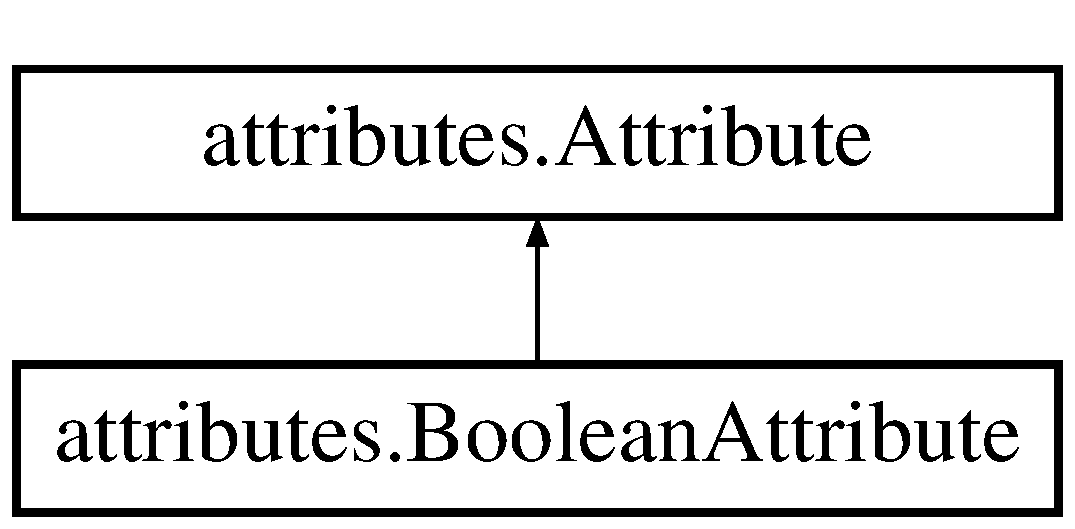
\includegraphics[height=2.000000cm]{classattributes_1_1_boolean_attribute}
\end{center}
\end{figure}
\subsection*{Public Member Functions}
\begin{DoxyCompactItemize}
\item 
\hypertarget{classattributes_1_1_boolean_attribute_a567a76969c4b7c4b14e36bd76b9ecb5b}{def {\bfseries initialize\-\_\-attribute}}\label{classattributes_1_1_boolean_attribute_a567a76969c4b7c4b14e36bd76b9ecb5b}

\end{DoxyCompactItemize}
\subsection*{Additional Inherited Members}


\subsection{Detailed Description}
Subclass of the \hyperlink{classattributes_1_1_attribute}{Attribute} Class. 

Use this if you know your Attribute\-String variable will be of the boolean type. 

The documentation for this class was generated from the following file\-:\begin{DoxyCompactItemize}
\item 
attributes.\-py\end{DoxyCompactItemize}

\hypertarget{classattributes_1_1_float_attribute}{\section{attributes.\-Float\-Attribute Class Reference}
\label{classattributes_1_1_float_attribute}\index{attributes.\-Float\-Attribute@{attributes.\-Float\-Attribute}}
}


Subclass of the \hyperlink{classattributes_1_1_attribute}{Attribute} Class.  


Inheritance diagram for attributes.\-Float\-Attribute\-:\begin{figure}[H]
\begin{center}
\leavevmode
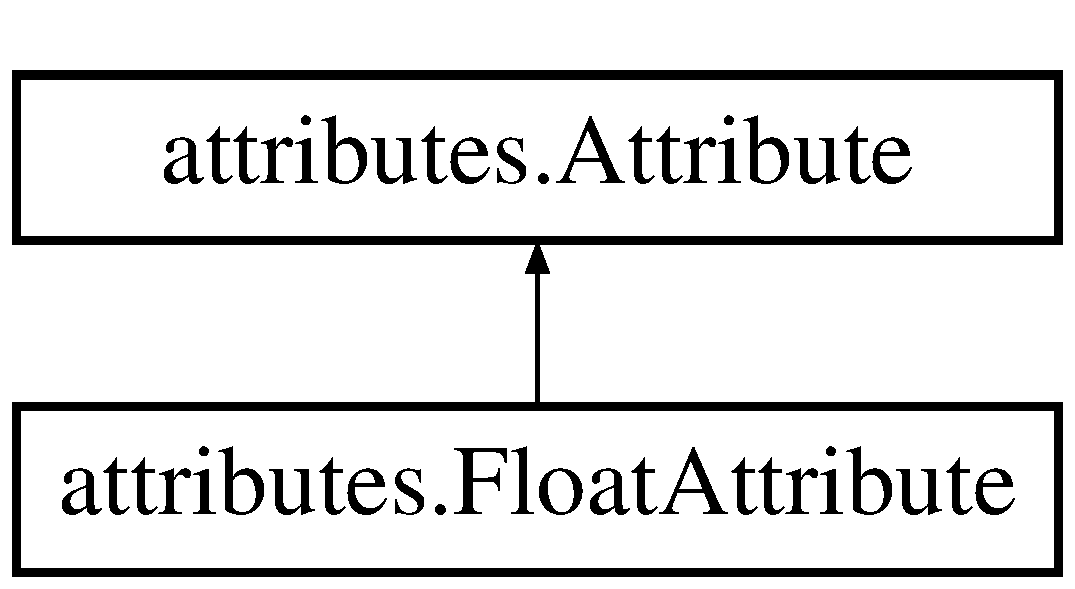
\includegraphics[height=2.000000cm]{classattributes_1_1_float_attribute}
\end{center}
\end{figure}
\subsection*{Public Member Functions}
\begin{DoxyCompactItemize}
\item 
\hypertarget{classattributes_1_1_float_attribute_ae7bff791c6736cc02774c795411f5260}{def {\bfseries initialize\-\_\-attribute}}\label{classattributes_1_1_float_attribute_ae7bff791c6736cc02774c795411f5260}

\end{DoxyCompactItemize}
\subsection*{Additional Inherited Members}


\subsection{Detailed Description}
Subclass of the \hyperlink{classattributes_1_1_attribute}{Attribute} Class. 

Use this if you know your Attribute\-String variable will be of the float type. 

The documentation for this class was generated from the following file\-:\begin{DoxyCompactItemize}
\item 
attributes.\-py\end{DoxyCompactItemize}

\hypertarget{classattributes_1_1_int_attribute}{\section{attributes.\-Int\-Attribute Class Reference}
\label{classattributes_1_1_int_attribute}\index{attributes.\-Int\-Attribute@{attributes.\-Int\-Attribute}}
}


Subclass of the \hyperlink{classattributes_1_1_attribute}{Attribute} Class.  


Inheritance diagram for attributes.\-Int\-Attribute\-:\begin{figure}[H]
\begin{center}
\leavevmode
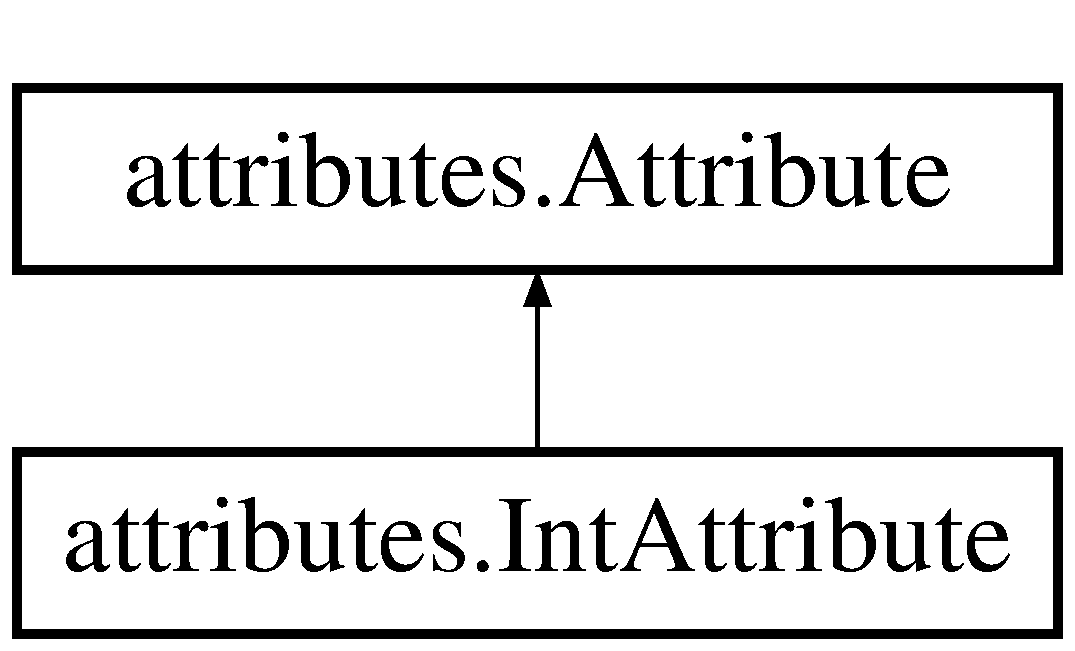
\includegraphics[height=2.000000cm]{classattributes_1_1_int_attribute}
\end{center}
\end{figure}
\subsection*{Public Member Functions}
\begin{DoxyCompactItemize}
\item 
\hypertarget{classattributes_1_1_int_attribute_a64a12f4797af23caaa241e857b567076}{def {\bfseries initialize\-\_\-attribute}}\label{classattributes_1_1_int_attribute_a64a12f4797af23caaa241e857b567076}

\end{DoxyCompactItemize}
\subsection*{Additional Inherited Members}


\subsection{Detailed Description}
Subclass of the \hyperlink{classattributes_1_1_attribute}{Attribute} Class. 

Use this if you know your Attribute\-String variable will be of the int type. 

The documentation for this class was generated from the following file\-:\begin{DoxyCompactItemize}
\item 
attributes.\-py\end{DoxyCompactItemize}

%--- End generated contents ---

% Index
\newpage
\phantomsection
\addcontentsline{toc}{chapter}{Index}
\printindex

\end{document}
